\documentclass[11pt,a4paper]{article}

\usepackage[T1]{fontenc}
\usepackage[utf8]{inputenc}
\usepackage[british]{babel}
\usepackage[left=0mm,right=0mm,top=0mm,bottom=0mm]{geometry}
\usepackage[stretch=25,shrink=25,tracking=true,letterspace=30]{microtype}
\usepackage{graphicx}
\usepackage{xcolor}
\usepackage{marvosym}
\usepackage{enumitem}
\setlist{parsep=0pt,topsep=0pt,partopsep=1pt,itemsep=1pt,leftmargin=6mm}
\usepackage{FiraSans}
\renewcommand{\familydefault}{\sfdefault}
\definecolor{cvblue}{HTML}{304263}

% --- Macros perso ------------------------------------------------------------
\newcommand{\dates}[1]{\hfill\mbox{\textbf{#1}}}
\newcommand{\is}{\par\vskip.5ex plus .4ex}
\newcommand{\smaller}[1]{{\small$\diamond$\ #1}}
\newcommand{\headleft}[1]{\vspace*{3ex}\textsc{\textbf{#1}}\par%
    \vspace*{-1.5ex}\hrulefill\par\vspace*{0.7ex}}
\newcommand{\headright}[1]{\vspace*{2.5ex}\textsc{\Large\color{cvblue}#1}\par%
     \vspace*{-2ex}{\color{cvblue}\hrulefill}\par}

\usepackage[colorlinks=true,urlcolor=white,linkcolor=white]{hyperref}

% -----------------------------------------------------------------------------

\begin{document}
\setlength{\topskip}{0pt}\setlength{\parindent}{0pt}\setlength{\parskip}{0pt}
\setlength{\fboxsep}{0pt}\pagestyle{empty}\raggedbottom

% ============================================================================
%                               COLONNE GAUCHE
% ============================================================================
\begin{minipage}[t]{0.33\textwidth}
\colorbox{cvblue}{\begin{minipage}[t][5mm][t]{\textwidth}\null\hfill\null\end{minipage}}
\vspace{-.2ex}
\colorbox{cvblue!90}{\color{white}
\kern0.09\textwidth
\begin{minipage}[t][293mm][t]{0.82\textwidth}\raggedright
\vspace*{2.5ex}

% ---- Identité ---------------------------------------------------------------
\Large Pape Saliou \textbf{\textsc{FALL}} \normalsize

\null\hfill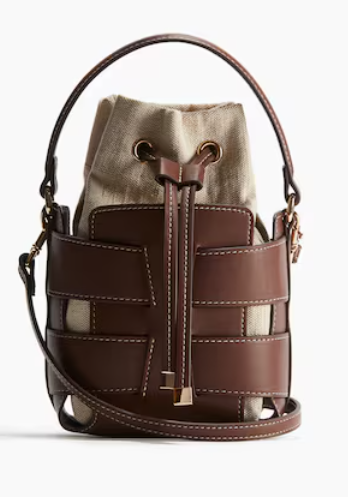
\includegraphics[width=0.65\textwidth]{ 311dccad0e264e6a971aa0a5a0caee16.png }\hfill\null

\vspace*{0.5ex}

% ---- Résumé -----------------------------------------------------------------
\headleft{Profile Summary}
Data Scientist passionné avec un solide bagage en statistiques, apprentissage automatique et analyse de données. Diplômé d’un Master 2 en Data Science de la Sorbonne, j’ai mené des projets de modélisation prédictive et de visualisation de données créant de la valeur pour l’entreprise. Curieux, orienté résultats et doté d’une forte capacité d’adaptation, je maîtrise l’ensemble du cycle de vie d’un projet data : collecte, nettoyage, exploration, modélisation, industrialisation et communication des insights.

% ---- Contact ----------------------------------------------------------------
\headleft{Contact details}\small
\MVAt\ {\small papesalioufall2@gmail.com} \\[0.4ex]
\Mobilefone\ 0753481453 \\[0.5ex]
\Letter\ Paris, France
\normalsize

% ---- Infos perso ------------------------------------------------------------
\headleft{Personal information}
Citizenship: \textbf{Française} \\[0.5ex]
Family: \textbf{Célibataire} \\[0.5ex]
Languages: \textbf{Français (natif), Anglais (courant)}

% ---- Compétences ------------------------------------------------------------
\headleft{Skills}
\begin{itemize}
  \item Python
  \item R
  \item SQL
  \item Machine Learning
  \item Deep Learning
  \item NLP
  \item Scikit-learn
  \item TensorFlow \& Keras
  \item PyTorch
  \item Spark
  \item Data Visualization (Tableau, Power BI, Plotly)
  \item Statistics
  \item Big Data
  \item Docker \& Kubernetes
  \item Git \& CI/CD
\end{itemize}

\end{minipage}\kern 0.09\textwidth
}
\end{minipage}
% ============================================================================
%                               COLONNE DROITE
% ============================================================================
\hskip2.5em
\begin{minipage}[t]{0.56\textwidth}
\setlength{\parskip}{0.8ex}
\vspace{2ex}

% ------------------------ EXPÉRIENCE ----------------------------------------
\headright{Experience}
\textsc{Data Scientist} at \textit{Prepaya} (Paris, France)  \dates{2022-2023} \\
\smaller{Développé des modèles prédictifs de churn client (Random Forest, XGBoost) augmentant la précision de 15 \%.}\is
\smaller{Mis en place un pipeline d’entraînement automatique sur AWS SageMaker réduisant le temps d’inférence de 30 \%.}\is
\smaller{Conçu des tableaux de bord interactifs sous Tableau pour le suivi des KPI business, améliorant la prise de décision.}\is
\smaller{Nettoyé et analysé des jeux de données volumineux (>50 M lignes) avec pandas et Spark.}\is
\smaller{Implémenté un système de versioning des données (DVC) et de déploiement continu via GitLab CI/CD.}\is
\smaller{Travaillé en méthodologie agile avec une équipe pluridisciplinaire (développeurs, marketing, produit).}\is

% ------------------------ ÉDUCATION ----------------------------------------
\headright{Education}
\textsc{Master 2 Data science}. \textit{Sorbonne Université}. \dates{2022-2023} \\

% ------------------------ CERTIFICATIONS ------------------------------------
\headright{Certifications}
\smaller{\textsc{TensorFlow Developer Certificate}}, \textit{DeepLearning.AI}. \dates{2023-05} \\
\smaller{\textsc{AWS Certified Machine Learning – Specialty}}, \textit{Amazon Web Services}. \dates{2024-02} \\

% ------------------------ HOBBIES -------------------------------------------
\headright{Hobbies}
\textit{Football, Échecs, Coding challenges, Lecture scientifique}

\end{minipage}

\end{document}